% !TeX program = xelatex

%%% Загружаем заголовочный файл, который хранит все настройки и все
%%% подгружаемые пакеты
\newcommand{\No}{\textnumero}

%%% Здесь выбираются необходимые графы
\documentclass[hpadding=3mm,russian,utf8,pointsection,simple]{styles/eskdtext}
\usepackage{fontspec}
\defaultfontfeatures{Mapping=tex-text} % Для того чтобы работали стандартные сочетания символов ---, --, << >> и т.п.

%%% Что бы работал eskdx и некоторые другие пакеты LaTeX
\usepackage{xecyr}

%%% Для работы шрифтов
\usepackage{xunicode}
\usepackage{xltxtra}

%%% Для работы с русскими текстами (расстановки переносов, последовательность комманд строго обязательна)
% \usepackage{polyglossia}
% \setdefaultlanguage{russian}
%\newfontfamily{\cyrillicfontt}{GOST_B}
%\set{GOST_type_A}
%\setmainfont{GOST_type_A.ttf}
%\setromanfont{GOST_type_A.ttf}
%\setsansfont{GOST_type_A.ttf}
%\setmonofont{GOST_type_A.ttf}
%
\setmainfont[
  BoldFont={Times_New_Roman_Bold.ttf},
  ItalicFont={Times_New_Roman_Italic.ttf},
  BoldItalicFont={Times_New_Roman_Bold_Italic.ttf}
]{Times_New_Roman.ttf}
\setromanfont[
  BoldFont={Times_New_Roman_Bold.ttf},
  ItalicFont={Times_New_Roman_Italic.ttf},
  BoldItalicFont={Times_New_Roman_Bold_Italic.ttf}
]{Times_New_Roman.ttf}
\setsansfont[
  BoldFont={Times_New_Roman_Bold.ttf},
  ItalicFont={Times_New_Roman_Italic.ttf},
  BoldItalicFont={Times_New_Roman_Bold_Italic.ttf}
]{Times_New_Roman.ttf}
\setmonofont[
  BoldFont={Times_New_Roman_Bold.ttf},
  ItalicFont={Times_New_Roman_Italic.ttf},
  BoldItalicFont={Times_New_Roman_Bold_Italic.ttf}
]{Times_New_Roman.ttf}

% polyglossia only
% \newfontfamily\cyrillicfont{GOST_type_A} 
% \newfontfamily\cyrillicfontrm{GOST_type_A}
% \newfontfamily\cyrillicfonttt{GOST_type_A}
% \newfontfamily\cyrillicfontsf{GOST_type_A}
%\defaultfontfeatures{Mapping=tex-text}


%%% Для работы со сложными формулами
\usepackage{amsmath}
\usepackage{amssymb}

%%% Что бы использовать символ градуса (°) - \degree
\usepackage{gensymb}


%%% Для переноса составных слов
%\XeTeXinterchartokenstate=1
\XeTeXcharclass `\- 24
\XeTeXinterchartoks 24 0 ={\hskip\z@skip}
\XeTeXinterchartoks 0 24 ={\nobreak}

%%% Ставим подпись к рисункам. Вместо «рис. 1» будет «Рисунок 1»
\addto{\captionsrussian}{\renewcommand{\figurename}{Рисунок}}
%%% Убираем точки после цифр в заголовках
\def\russian@capsformat{%
  \def\postchapter{\@aftersepkern}%
  \def\postsection{\@aftersepkern}%
  \def\postsubsection{\@aftersepkern}%
  \def\postsubsubsection{\@aftersepkern}%
  \def\postparagraph{\@aftersepkern}%
  \def\postsubparagraph{\@aftersepkern}%
}



% Автоматически переносить на след. строку слова которые не убираются
% в строке
\sloppy

%%% Для вставки рисунков
\usepackage{graphicx}
\graphicspath{ {images/} }

%%% Для вставки интернет ссылок, полезно в библиографии
\usepackage{url}

%%% Подподразделы(\subsubsection) не выводим в содержании
\setcounter{tocdepth}{2}

%%% Большие таблицы
\usepackage{longtable}

%%% Отключение отступов в перечислениях
%\usepackage{enumitem}
%\setlist[itemize]{noitemsep, topsep=0pt}
%\setlist[enumerate]{noitemsep, topsep=0pt}


%%% Каждый раздел (\section) с новой страницы
\let\stdsection\section
\renewcommand\section{\newpage\stdsection}

%%% Загружаем настройки пакета eskdx, там нужно заполнить информацию
%%% о документе - ФИО авторов, название документов и т.п.
%%% Название документа
\ESKDtitle{ УЧЕБНАЯ ПРАКТИКА }%TODO
\ESKDdocName{ Пояснительная записка }

\ESKDauthor{ Копорушкин Л.Н. }
\ESKDchecker{ Сухоева К.С. }
%\ESKDnormContr{ Н.Кнтр.~И.О. }
%\ESKDnormContr{ Н.Кнтр.~И.О. }

%%% Для титульника
%\ESKDtitleApprovedBy{ Должность утверждающего }{ Фам. утвер. }
%\ESKDtitleAgreedBy{ Должность первого согласовавшего }{ Фам. первого согл. }
%\ESKDtitleAgreedBy{ Должность второго согласовавшего }{ Фам. второго согл. }
%\ESKDtitleAgreedBy{ Должность третьего согласовавшего }{ Фам. третьего согл. }
%\ESKDtitleDesignedBy{ Должность первого автора }{ Фам. первого автора }
%\ESKDtitleDesignedBy{ Должность второго автора }{ Фам. второго автора }

\ESKDdepartment{ Министерство цифрового развития, связи и массовых коммуникаций РФ }
\ESKDcompany{ Федеральное государственное бюджетное образовательное учреждение высшего образования «Сибирский государственный университет телекоммуникаций и информатики» (СибГУТИ) Уральский технический институт связи и информатики (филиал) в г. Екатеринбурге (УрТИСИ СибГУТИ) }
\ESKDgroup{ УрТИСИ СибГУТИ }
\ESKDdiplomaName{ Модернизация системы видеонаблюдения 4 этажа 3 корпуса УрТИСИ СибГУТИ }
\ESKDsignature{  }

\ESKDdate{ 2025/3/3 }
% TODO

\begin{document}
    %%% Делаем содержание
    \tableofcontents

    %%% Введение пишется без цифры и добавляется в содержание
    \section*{Введение}
\addcontentsline{toc}{section}{Введение}

В современном мире обеспечение безопасности является одной из ключевых задач для образовательных учреждений.
Системы видеонаблюдения играют важную роль в создании безопасной инфраструктуры и
повышении уровня защиты студентов и сотрудников.
Однако, с учетом динамичного развития технологий, существующие системы могут требовать обновлений и
модернизации для соответствия современным требованиям.

Настоящий проект направлен на модернизацию системы видеонаблюдения на четвертом этаже
третьего корпуса Уральского государственного технического университета.

Работа включает в себя анализ текущего состояния системы, изучение современных технологий видеонаблюдения
и разработку рекомендаций по их внедрению.
В результате предполагается повысить эффективность работы системы видеонаблюдения, улучшить качество изображения,
обеспечить удобство доступа к видеоданным и повысить уровень безопасности на данном этаже.

Данная модернизация не только обеспечит более надежный контроль, но и создаст комфортные условия для учебного процесса,
способствуя созданию безопасной и эффективной образовательной среды.
    \section{Описание объекта}

\begin{figure}[h]
    \begin{center}
        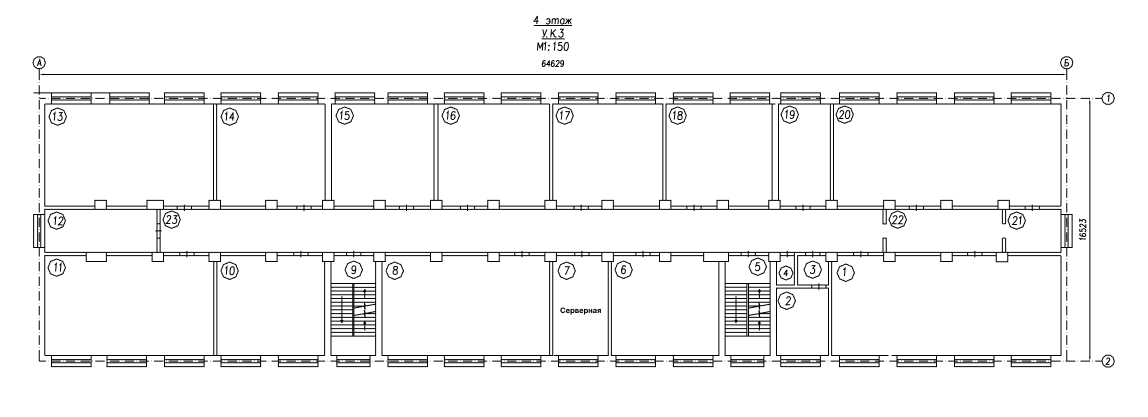
\includegraphics[width=180mm]{images/План объекта}
    \end{center}
    \captionsetup{justification=centering}
    \caption{План объекта}
    \label{fig::object_placement}
\end{figure}

\begin{longtable}{|p{5cm}|p{3cm}|p{8cm}|}
    \caption{Описание помещений на объекте}
    \label{tab::rooms_description} \\

    \hline
    Номер помещения &
    Площадь, м2 &
    Назначение \\
    \hline
    1 &
    96 &
    Учебное помещение \\
    \hline
    2 &
    14 &
    Служебное помещение \\
    \hline
    3 &
    3 &
    Служебное помещение \\
    \hline
    4 &
    2 &
    Служебное помещение \\
    \hline
    5 &
    - &
    Лестничная площадка \\
    \hline
    6 &
    44 &
    Учебное помещение \\
    \hline
    7 &
    22 &
    Серверная \\
    \hline
    8 &
    69 &
    Учебное помещение \\
    \hline
    9 &
    - &
    Лестничная площадка \\
    \hline
    10 &
    44 &
    Учебное помещение \\
    \hline
    11 &
    69 &
    Учебное помещение \\
    \hline
    12 &
    20 &
    Служебное помещение \\
    \hline
    13 &
    69 &
    Учебное помещение \\
    \hline
    14 &
    44 &
    Учебное помещение \\
    \hline
    15 &
    44 &
    Учебное помещение \\
    \hline
    16 &
    44 &
    Учебное помещение \\
    \hline
    17 &
    44 &
    Учебное помещение \\
    \hline
    18 &
    44 &
    Учебное помещение \\
    \hline
    19 &
    22 &
    Служебное помещение \\
    \hline
    20 &
    96 &
    Учебное помещение \\
    \hline
    21 &
    9 &
    Коридор \\
    \hline
    22 &
    20 &
    Коридор \\
    \hline
    23 &
    129 &
    Коридор \\
    \hline
\end{longtable}
    \section{Определение задач проекта видеонаблюдения}

Система видеонаблюдения предназначена для выполнения основных задач:

\begin{enumerate}
    \item Повышение эффективности обеспечения пропускного и внутри объектового режима, антитеррористической защищённости;
    \item Обеспечение и контроль качества и безопасности деятельности внутри объекта;
    \item Оценка и контроль данных обстановки, анализ обстановки, принятых мер по ликвидации нештатных ситуации, уточнение и корректировка по обстановке заранее разработанных вариантов решений по ликвидации каждой типовой нештатной ситуации;
    \item Получение информации о текущем состоянии объектов, анализ и оценка достоверности поступившей информации, доведение ее до руководства;
    \item Обеспечение противопожарной защиты помещений, зданий, сооружений и территории;
    \item Повышение эффективности действий при возникновении нештатных и чрезвычайных ситуаций, оповещения студентов (получателей/потребителей образовательных услуг) и работников об угрозе возникновения чрезвычайных ситуаций, необходимых действиях по эвакуации;
    \item Отслеживание, фиксация обстоятельств и фактов в целях недопущения и минимизации рисков материальных потерь, имущества в УрТИСИ СибГУТИ, сохранность личного имущества работников, имущества контрагентов и студентов (получателей/потребителей образовательных услуг), несанкционированного проникновения в служебные помещения, ущерба здоровью людей;
    \item Фиксация возможных противоправных действий, которые могут нанести вред имуществу. В случае необходимости материалы видеозаписей, полученных камерами видеонаблюдения, могут быть переданы и использованы в качестве доказательства соответствующими службами и государственными органами в случаях, предусмотренных действующим законодательством РФ для доказывания факта совершения противоправного действия, а также для установления личности лица, совершившего соответствующее противоправное действие;
    \item Осуществление контроля трудовой дисциплины и обеспечение объективности при вынесении дисциплинарных взысканий для доказывания факта совершения дисциплинарного проступка работником;
    \item Осуществление контроля в условиях, где другими средствами обеспечить его невозможно;
    \item Предоставление информации по официальным запросам соответствующих служб и государственных органов в случаях, предусмотренных действующим законодательством РФ;
\end{enumerate}

    \section{Описание существующей системы видеонаблюдения}


    \section{Разработка технического задания на модернизацию системы видеонаблюдения}

\subsection{Выбор топологии}

При топологии «звезда» каждая камера подключается по 1 кабелю к общему сетевому оборудованию (коммутатор, маршрутизатор).
Среди основных достоинств такой топологии расширяемость и управляемость. подводится к ее низкая стоимость, легкость подключения, отличная модернизация СКС.
Недостатки топологии «звезда», предполагает достаточно высокую стоимость внедрения и большое количество кабеля, а при отказе сетевого оборудования от сети 
отключаются все подцепленные к нему устройства системы видеонаблюдения.

\subsection{Выбор и описание параметров видеооборудования}

Видеооборудование было выбрано от компании TRASSiR\@.
Компания TRASSiR является одним из ведущих разработчиков решений в области информационных технологий и автоматизации процессов мониторинга и управления.
Основанная в 2007 году, TRASSiR сосредоточена на разработке и внедрении программных продуктов, предназначенных для повышения эффективности работы организаций различных отраслей.

Была выбрана модель видеокамеры TR-D2D2 v3 2.7-13.5, т.к. она подходит по основным необходимым параметрам.
Внешний вид видеокамеры показан на рисунке~\ref{fig::tr-d2d2}:

\begin{figure}[h]
    \begin{center}
        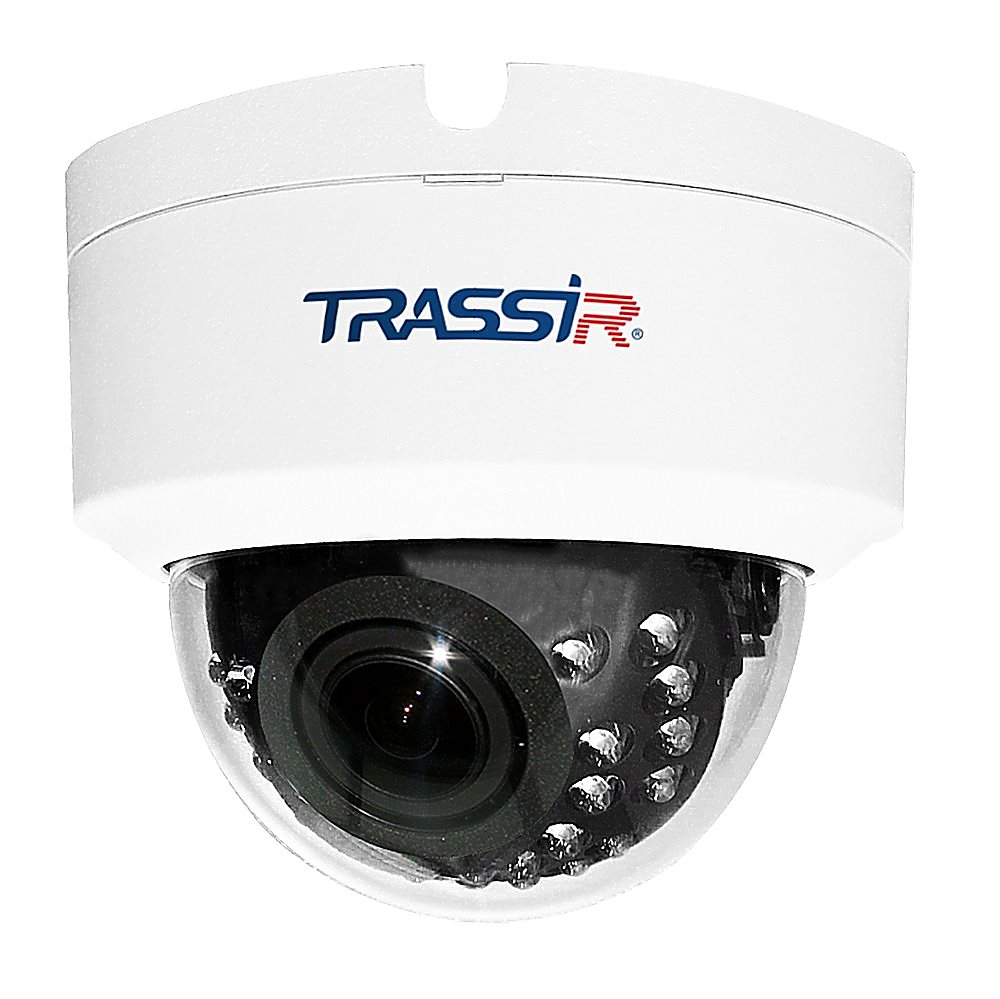
\includegraphics[width=50mm]{images/TR-D2D2}
    \end{center}
    \captionsetup{justification=centering}
    \caption{Внешний вид видеокамеры TR-D2D2}
    \label{fig::tr-d2d2}
\end{figure}

Технические характеристики указаны в таблице~\ref{tab::tr-d2d2-parameters}:
\begin{longtable}{|p{5cm}|p{12cm}|}
    \caption{Технические характеристики видеокамеры TR-D2D2 v3 2.7-13.5}
    \label{tab::tr-d2d2-parameters} \\

    \hline
    Параметр &
    Данные \\
    \hline
    Класс защиты &
    Нет \\
    \hline
    Детектор движения &
    Да \\
    \hline
    Кнопка сброса &
    Нет \\
    \hline
    Локальное хранилище &
    Нет \\
    \hline
    Улучшение изображения &
    3D DNR | BLC | Defog \\
    \hline
    Число пикселей &
    2 Мп \\
    \hline
    Тип объектива &
    С переменным фокусным расстоянием \\
    \hline
    Фокусное расстояние, мм &
    2.7 - 13.5 \\
    \hline
    Угол обзора H° &
    100 - 28 \\
    \hline
    Угол обзора V° &
    55 - 16 \\
    \hline
    Угол обзора D° &
    Нет \\
    \hline
    Сетевой интерфейс &
    RJ-45 \\
    \hline
    Видеосжатие &
    H.264, H.265, H.265+ \\
    \hline
    Поддержка RTSP &
    Да \\
    \hline
    Матрица &
    1/2.9'' CMOS \\
    \hline
    Максимальное разрешение &
    1920x1080 \\
    \hline
    Светочувствительность, Lux &
    0,003 \\
    \hline
    Питание &
    DC 12 В, PoE \\
    \hline
\end{longtable}

\newpage

В качестве коммутатора был выбран коммутатор от компании TRASSiR TR-NS1126-225-24PoE.
Внешний вид видеокамеры показан на рисунке~\ref{fig::TR-NS1126-225-24PoE}:

\begin{figure}[h]
    \begin{center}
        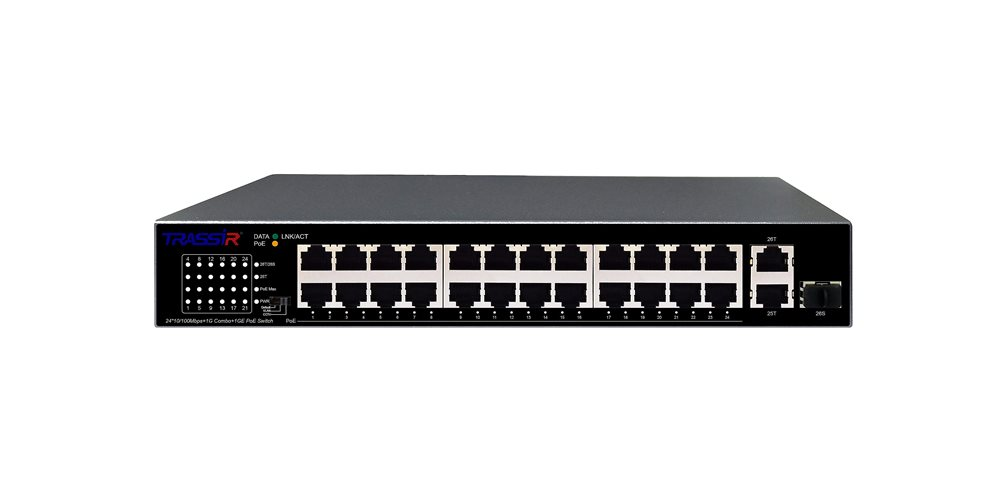
\includegraphics[width=120mm]{images/TR-NS1126-225-24PoE}
    \end{center}
    \captionsetup{justification=centering}
    \caption{Внешний вид коммутатора TR-NS1126-225-24PoE}
    \label{fig::TR-NS1126-225-24PoE}
\end{figure}

Технические характеристики указаны в таблице~\ref{tab::TR-NS1126-225-24PoE-parameters}:
\begin{longtable}{|p{5cm}|p{12cm}|}
    \caption{Технические характеристики коммутатора ЕR-NS1126-225-24PoE}
    \label{tab::TR-NS1126-225-24PoE-parameters} \\

    \hline
    Параметр &
    Данные \\
    \hline
    Управление &
    Нет \\
    \hline
    Таблицы MAC-адресов, К &
    16 \\
    \hline
    Скорость обслуживания пакетов, Mpps &
    6,5 \\
    \hline
    Способ монтажа &
    В стойку / на плоскую поверхность \\
    \hline
    Питание &
    DC 55 В \\
    \hline
    Количество портов PoE &
    24 \\
    \hline
    Количество SFP портов &
    1 \\
    \hline
\end{longtable}

\newpage
В качестве видеорегистратора был выбран коммутатор от компании TRASSiR DuoStation AF Pro 16-RE
Внешний вид видеорегистратора показан на рисунке~\ref{fig::recorder}:

\begin{figure}[h]
    \begin{center}
        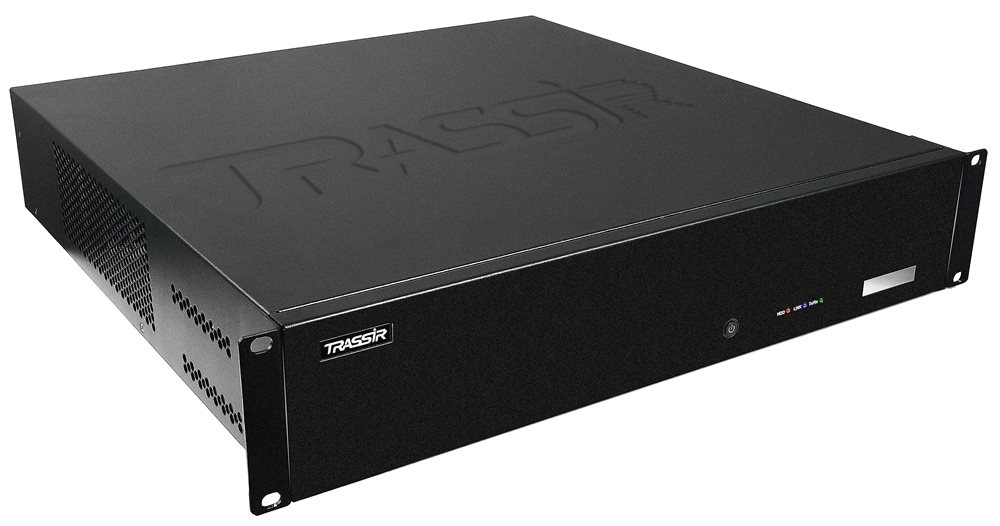
\includegraphics[width=80mm]{images/DuoStation AF Pro 16-RE}
    \end{center}
    \captionsetup{justification=centering}
    \caption{Внешний вид видеорегистратора DuoStation AF Pro 16-RE}
    \label{fig::recorder}
\end{figure}

Технические характеристики указаны в таблице~\ref{tab::recorder-parameters}:
\begin{longtable}{|p{5cm}|p{12cm}|}
    \caption{Технические характеристики видеорегистратора DuoStation AF Pro 16-RE}
    \label{tab::recorder-parameters} \\

    \hline
    Параметр &
    Данные \\
    \hline
    Формат видеосжатия &
    H.265+ | H.265 | H.264 | MJPEG | MPEG4 \\
    \hline
    Объем HDD, TB &
    16 \\
    \hline
    Сетевые протоколы &
    TCP/IP, IPv4/v6, UDP, DHCP, CloudConnect, DNS, NTP, SADP, SMTP, iSCSI, UPnP, HTTP/HTTPS, RTSP, ONVIF \\
    \hline
    Сетевые интерфейсы &
    2 RJ-45 10M/100M/1000M Ethernet \\
    \hline
    Кол-во IP каналов &
    16 \\
    \hline
    Основной поток записи, Мп &
    8 \\
    \hline
    Количество SFP портов &
    1 \\
    \hline
\end{longtable}

\subsection{Разработка плана размещения видеокамер}

Размещение видеокамер на объекте было рассчитано с учетом технических характеристик выбранных камер. 
На помещения с площадью меньше 22 м^2 выделено по 1 видеокамере направленной из 1 угла комнаты в сторону входной двери, для её контроля. 
На помещения превышающие площадь 22 м^2 используется по 2 видеокамеры направленных друг на друга с целью предотвращения умышленного 
перекрывания видеонаблюдения нарушителем. Одна из камер обязательно должна иметь прямую видимость входной двери и дверного проема, 
для контроля входящих в помещение работников и студентов. Исключением является помещение под номером 12, потому что подразумевается как 
помещение для работников, в котором возможно будут храниться ценные вещи. Коридор разделен на 3 части, в каждой части коридора имеется 
по 2 видеокамеры направленных друг на друга с целью контроля состояния видеокамер и области вокруг/за видеокамерой. Такая расстановка 
видеокамер увеличивает безопасность имущества и покрывает большую часть охраняемой области. Общее число используемых видеокамер составляет 
34 штуки. К 1 коммутатору подключено 17 видеокамер, используется 2 коммутатора для подключения к видеокамерам и 1 коммутатор для объединения 
потока информации и передачи на основной сервер.

\begin{sidewaysfigure}
    \begin{center}
        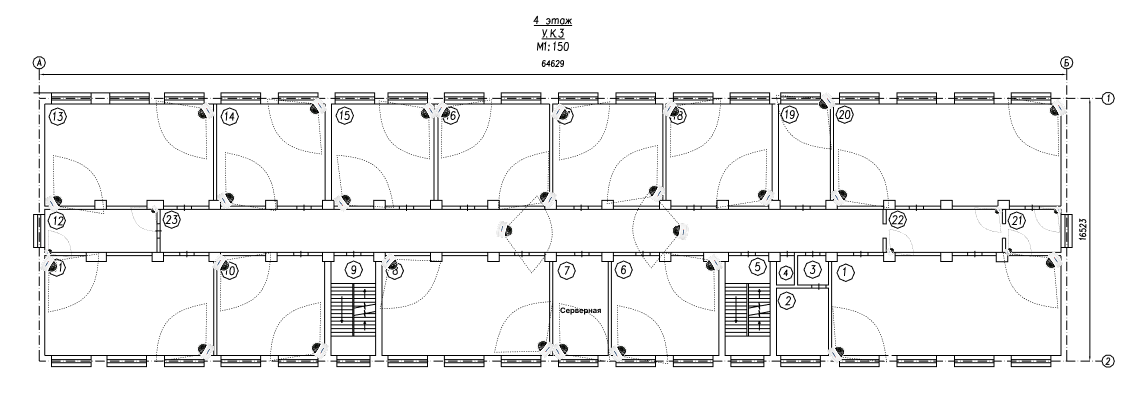
\includegraphics[width=240mm]{images/План размещения видеокамер}
    \end{center}
    \captionsetup{justification=centering}
    \caption{План размещения видеокамер}
    \label{fig::videocameras_placement}
\end{sidewaysfigure}


\subsection{Разработка схемы подключения оборудования}

\begin{figure}[h]
    \begin{center}
        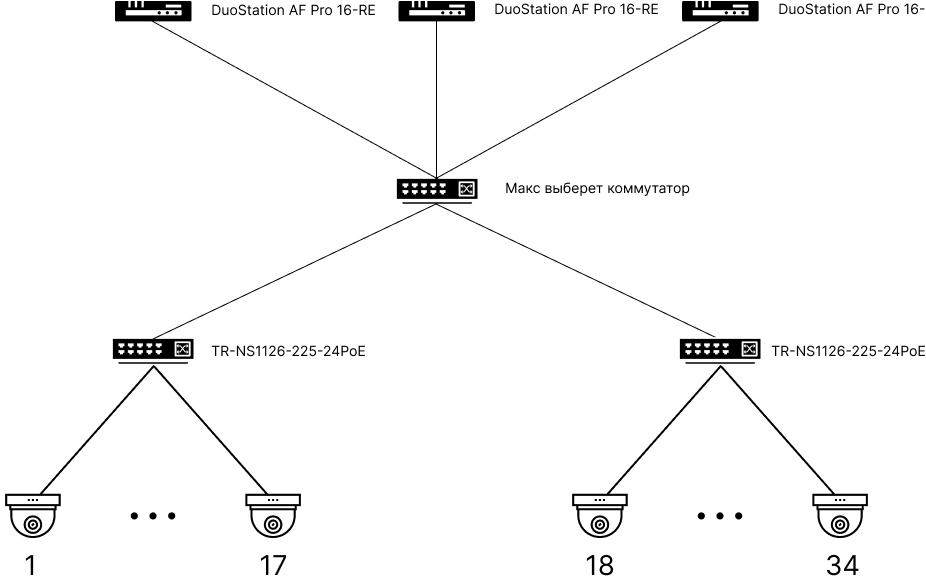
\includegraphics[width=160mm]{images/Схема подключения оборудования}
    \end{center}
    \captionsetup{justification=centering}
    \caption{Схема подключения оборудования}
    \label{fig::connections}
\end{figure}

    \section*{Заключение}
\addcontentsline{toc}{section}{Заключение}

В результате проведенной практической работы была успешно модернизирована система видеонаблюдения 
4-го этажа 3-го корпуса УрТИСИ СибГУТИ. Проведенный анализ существующих слепых зон позволил оптимизировать 
расположение камер и расширить систему путем добавления новых устройств.
Ключевые результаты модернизации:
\begin{enumerate}
    \item Улучшение покрытия: Установка дополнительных камер и корректировка углов обзора существующих позволила устранить все выявленные слепые зоны. Теперь вся территория 4-го этажа находится под постоянным видеонаблюдением.
    \item Повышение безопасности: Расширенная система видеонаблюдения значительно повышает уровень безопасности объекта, обеспечивая круглосуточный контроль за происходящим.
    \item Улучшение качества изображения: Замена устаревших камер на современные модели с высоким разрешением обеспечила более четкое и детализированное изображение, что облегчает идентификацию объектов и событий.
    \item Возможность дальнейшего расширения: Модернизированная система обладает гибкой архитектурой, позволяющей в будущем добавлять новые камеры и интегрировать дополнительные функции, такие как аналитика видеопотока.
\end{enumerate}
В целом, модернизация системы видеонаблюдения 4-го этажа 3-го корпуса УрТИСИ СибГУТИ позволила создать эффективную и надежную систему, отвечающую современным требованиям безопасности.


    %%% Библиография
    \catcode`"\active\def"{\relax}
    \bibliographystyle{styles/ugost2008}
    \bibliography{bibliography}
\end{document}
